\chapter{Atividades Realizadas}

\section{Protótipo das implementações do método}
A implementação do método foi toda feita utilizando orientação a objetos em C++, com excessão das funções específicas ao cálculo que possuem implementações, em CUDA, OpenCL e C++. Estas funções específicas ao cálculo consistem de operações básicas com vetores, aproximações para o campo vetorial e o método de Runge-Kutta em si. O código compartilhado entre as demais implementações vai desde as estruturas de dados até representações dos resultados em OpenGL.

O código pode ser encontrado em seu repositório Git \newline(em \href{https://github.com/rafamanzo/runge-kutta}{https://github.com/rafamanzo/runge-kutta}) é organizado basicamente em quatro pastas:
\begin{itemize}
  \item \textbf{core} contém as três implementações do método nas pastas \textit{c}, \textit{cuda} e \textit{opencl}; além das estruturas de dados que repensentam a entrada (\textit{dataset.cpp}) e a saída do método (\textit{fiber.cpp}).
  \item \textbf{example-factories} contém os scripts que geram arquivos de entrada para o protótipo de campos vetoriais sintéticos como exemplos;
  \item \textbf{includes} contém todos os cabeçalhos necessários, facilitando sua inclusão;
  \item \textbf{io} contém as classes que cuidam da entrada e saída do protótipo. A pasta \textit{gui} contém as abstrações utilizadas para a criação de uma interface gráfica com Glut e OpenGL.
\end{itemize}

\newpage
As interações entre todas as classes que compõe o protótipo podem ser vistas através do seguinte diagrama de classes:
\begin{figure}[!h]
  \begin{center}
    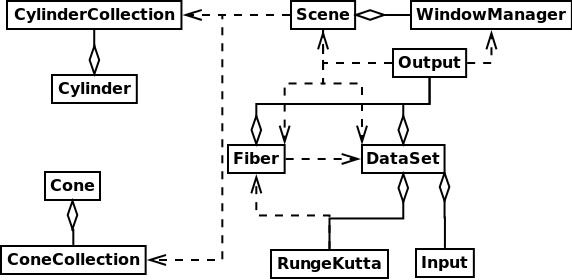
\includegraphics[width=120mm, height=60mm]{images/diagramadeclasse.png}
    \label{fig:}
    \caption{Diagrama de classes simplificado para o protótipo}
  \end{center}
\end{figure}

  \subsection{Estruturas compartilhadas em C++}
  A estrutura mais básica é a \textit{vector} contida em \textit{include/dataset.h}, consistindo de três \textit{doubles}. Sua responsabilidade é representar tanto vetores quanto pontos no $\Re ^{3}$. Neste mesmo arquivo também está a representação da classe \textit{DataSet}, cujo uso é representar as informações de entrada referentes ao campo vetorial e encapsular seu acesso. Analogamente, a classe \textit{Fiber} é responsável por representar os resultados da aplicação do algoritmo.
  
  Além destas abstrações de entrada e saída, existem classes que de fato são responsáveis pela entrada e saída do protótipo. A mais simples é a classe que cuida da entrada, \textit{Input}, que possui os métodos para ler um arquivo de texto que contenha as informações sobre o campo vetorial, pontos iniciais e tamanho de passo (conforme descrito no arquivo \textit{README} que acompanha o protótipo). Outra opção de entrada é o formato Analyze que é suportado pelo biblioteca $\textit{CImg}_{\ref{CImg}}$ e portanto o método da classe \textit{Input} que processa este tipo de entrada apenas faz uma chamada a esta biblioteca.
  
  Por fim, a última estrutura compartilhada entre as três implementações é a saída. A forma mais simples de visualizar os resultados é através do $\textit{gnuplot}_{\ref{gnuplot}}$ passando para este o arquivo \textit{rk2-vs-rk4} que é criado ao fim da execução do algoritmo. Por outro lado, a saída pode ser bastante mais complexa que apenas uma classe, como é a entrada, devido à visualização com \textit{Glut} e \textit{OpenGL}.
  
  Esta visualização é composta das classes, aqui denomidas como primitivas, que contém representações de cilindros e cones (classes \textit{Cylinder} e \textit{Cone}) e as responsáveis por representar coleções destas classes (\textit{CyllinderCollection} e \textit{ConeCollection}). Estas classes primitivas contém principalmente informações sobre como renderizar estes objetos.
  
  Por fim, ainda na interface gráfica, existe a classe \textit{Scene} que é responsável por fornecer métodos que utilizam as primitivas para evitar que a classe \textit{WindowManager} use diretamente as primitivas e tenha que conhecer suas especificidades. Ou seja, ela é como uma camada de abstração para a \textit{WindowManager}, permitindo que esta seja responsável apenas pela interação com a \textit{Glut}. 
  
  \subsection{Implementação do método}
  A implementação em cada linguagem pode ser encontrada nas subpastas de \textit{core} (\textit{c}, \textit{cuda} e \textit{opencl}), nos arquivos \textit{rk\_kernel.*} aos quais iremos nos referir apenas como \textit{kernel}. Também cada uma destas pastas contém um arquivo \textit{rk.cpp} reponsável por fornecerer uma interface para seu respectivo \textit{kernel}.
  
  Estas interfaces são utilizadas pois a implementação, por limitação do \textit{CUDA} e do \textit{OpenCL}, não pode ser feita utilizando orientação a objetos. Então a classe (\textit{RungeKutta}) implementada no arquivo \textit{rk.cpp} é a responsável por encapsular o conjunto de funções definidas em seu respectivo \textit{kernel}.

  Cada arquivo de \textit{kernel}, além de conter a implementação do método, possui funções auxiliares para se trabalhar com elementos do $\Re ^{3}$ (soma, subtração, módulo, distância e produto por um escalar) e as funções de aproximação necessárias (\ref{aproximacao}).
  
  Com toda esta estrutura descrita, o método em si é a simples implementação do que é descrito para as ordens 2 e 4 na seção \ref{rungekutta} com especificidades para as diferentes linguagens utilizadas descritas a seguir.
  
  Antes é preciso destacar que todas as implementações de diferentes ordens são funções independentes umas das outras e que, para evitar que falte memória, os resultados foram limitados a 10000 pontos que podem ser gerados a partir de cada ponto inicial.
  
    \subsubsection{Observações sobre o método em C++}
    Esta implementação, ao contrário das demais, foi feita sequencial e apenas não foi feita orientada a objetos para seguir a arquitetura necessária para as outras duas implementações.
    
    \subsubsection{Observações sobre o método em CUDA}
    Nesta implementação para \textit{GPU}, além do limite de 10000 pontos que podem ser gerados por cada ponto, é feita uma rechecagem após alocar toda a memória necessária para o \textit{DataSet} calculando novamente a quantidade máxima de pontos que podem ser gerados a partir de cada ponto inicial baseado na memória dedicada que restou. Então, o limite é o mínimo entre 10000 e este valor calculado.
    Outro ponto importante de destacar é que a chamada é feita com apenas um bloco contendo uma \textit{thread} para cada ponto inicial sobre o qual o algoritmo deverá ser aplicado.
    
    \subsubsection{Observações sobre o método em OpenCL}
    
  \subsection{Geração de campos vetoriais sintéticos}
  Campos vetoriais extensos ocupam muito espaço em disco, mesmo, compactados para serem distribuídos de forma prática junto do protótipo. Então, para torna-los disponíveis junto com o protótipo, foram escritos scripts \textit{PHP} que os geram todos eles contidos dentro da pasta \textit{example-factories}.
  
  O campo mais simples gerado possui dimensões 128x128x20, representando uma rotação sobre o eixo z. Nele, o método é aplicado com tamanho de passo 0.1 e pontos iniciais: (0, 16, 10); (0, 32, 10); (0, 48, 10); (0, 64, 10); (0, 80, 10); (0, 96, 10); e  (0, 112, 10). O segundo campo é uma inversão periódica no sentido da coordenada y, num campo de tamanho 512x512x128. A aplicação do método sobre ele se dá com tamanho de passo 0.2 e tem um único ponto inicial: (0, 64, 64).
  
  Os dois campos anteriores são úteis para vrificar se o método se comporta como esperado, mas são pouco úteis para medir a performance e não reproduzem uma variedade de casos. Portanto, os dois exemplos a seguir procuram suprir estas carências.
  
  O terceiro exemplo é um campo com direções aleatórias com dimensão 256x256x256. Para este campo o método é aplicado com tamanho de passo 0.1 e também são criados 256 pontos iniciais com posições aleatórias.
  
  Por fim, no último campo as direções possuem uma distribuição normal com média 10 e variância 1 e sua dimensão é 256x256x256. Ele possui um único ponto inicial aleatório e tamanho de passo 0.1.

\section{Protótipo das implementações utilizando a biblioteca VTK}
\section{Comparação de perfomance entre as implementações}
Foram feitas comparações entre as implementações do método para CPU utilizando \textit{POSIX threads} com o método para GPU em CUDA. Estes resultados foram obtidas em duas CPUs Intel e GPUs NVIDIA diferentes a fim de comprovar o que foi afirmado anteriormente sobre os desempenhos do método em cada um destes ambientes.

  \subsection{Metodologia}
    \subsubsection{Dados de entrada}
    Para isto foi gerado um campo vetorial sintético com dimensões de 512 pontos no eixo x, 256 pontos no eixo y e outros 256 pontos no eixo z. Todos com o mesmo vetor direção $(0, 1, 0)$ e até 512 pontos iniciais da forma $(x, 0, 128)$, onde $0 \leq x \leq 512$.
    
    Os testes foram realizados para os primeiros 16, 32, 64, 128 e 256 pontos iniciais a fim de se obter como que o método escala em cada um dos ambientes.
    
    \subsubsection{Medições de tempo}
    A medição de tempo é dividida em tempo consumido por operações em memória (alocação e transferência) e processamento do método. Sempre realizando a contagem de \textit{clocks} em cada um dos ambientes.
    
    \subsubsection{Casos}
    Cada medição consistiu em executar, trinta vezes cada implementação para estes dados (restringindo a quantidade de pontos iniciais conforme descrito), obtendo a média e desvio padrão do tempo em segundos consumidos em operações de transferência de dados, alocação de memória e processamento dos pontos que compõe a trajetória.    

  \subsection{Resultados em CPU}
  Foram realizados os testes em duas CPUs Intel diferentes:
  \begin{itemize}
    \item Core 2 Duo E7400, com dois núcleos físicos e lógicos a 2.8GHz cada;
    \item Core i7-2620M, com quatro núcleos físicos e lógicos a 2.7GHz cada.
  \end{itemize}
  
  O primeiro utiliza dois módulos de memória DDR2 em Dual Channel, enquanto que o segundo utiliza dois módulos de memória DDR3 em Dual Channel.
    \subsubsection{Runge-Kutta Ordem 2}
    Média dos tempos de execução para processamento em segundos:\\
    \begin{tabular}{| c | c | c | c | c | c |}
      \hline
      \multirow{2}{*}{Processadores}& \multicolumn{5}{|c|}{Quantidade de pontos iniciais} \\ \cline{2-6}
      & 16 & 32 & 64 & 128 & 256 \\ \hline
      Core 2 Duo & 1.142000 & 4.092000 & 16.435333 & 62.781000 & 302.174000 \\ \hline
      Core i7 & 2.142667 & 7.820000 & 35.778333 & 148.151000 & 604.198333\\ \hline

      \hline
    \end{tabular}
    
    \hspace{1mm}\newline
    
    \noindent Desvio padrão dos tempo de execução para processamento em segundos:\\
    \begin{tabular}{| c | c | c | c | c | c |}
      \hline
      \multirow{2}{*}{Processadores}& \multicolumn{5}{|c|}{Quantidade de pontos iniciais} \\ \cline{2-6}
      & 16 & 32 & 64 & 128 & 256 \\ \hline
      Core 2 Duo & 0.066403 & 0.131108 & 0.241809 & 1.270736 & 15.763295 \\ \hline
      Core i7 &  0.160933 & 0.572346 & 0.807395 & 1.323819 & 7.807908 \\ \hline

      \hline
    \end{tabular}
    
    \hspace{1mm}\newline
    
    \noindent Média dos tempos de execução para operações em memória em segundos:\\
    \begin{tabular}{| c | c | c | c | c | c |}
      \hline
      \multirow{2}{*}{Processadores}& \multicolumn{5}{|c|}{Quantidade de pontos iniciais} \\ \cline{2-6}
      & 16 & 32 & 64 & 128 & 256 \\ \hline
      Core 2 Duo & 2.118667 & 2.115333 & 2.109667 & 1.059667 & 2.120000 \\ \hline
      Core i7 & 1.041333 & 1.063333 & 1.063667 & 1.118000 & 1.075333\\ \hline

      \hline
    \end{tabular}
    
    \hspace{1mm}\newline
    
    \noindent Desvio padrão dos tempo de execução para operações em memória em segundos:\\
    \begin{tabular}{| c | c | c | c | c | c |}
      \hline
      \multirow{2}{*}{Processadores}& \multicolumn{5}{|c|}{Quantidade de pontos iniciais} \\ \cline{2-6}
      & 16 & 32 & 64 & 128 & 256 \\ \hline
      Core 2 Duo & 0.066403 & 0.014314 & 0.011075 & 0.011431 & 0.011255 \\ \hline
      Core i7 & 0.052009 & 0.011643 & 0.807395 & 0.018345 & 0.023055 \\ \hline

      \hline
    \end{tabular}
    
    \subsubsection{Runge-Kutta Ordem 4} 
    Média dos tempos de execução para processamento em segundos:\\
    \begin{tabular}{| c | c | c | c | c | c |}
      \hline
      \multirow{2}{*}{Processadores}& \multicolumn{5}{|c|}{Quantidade de pontos iniciais} \\ \cline{2-6}
      & 16 & 32 & 64 & 128 & 256 \\ \hline
      Core 2 Duo & 1.309333 & 4.340333 & 16.764333 & 62.903667 & 294.720000 \\ \hline
      Core i7 & 1.810333 & 7.136667 & 33.477333 & 138.473333 & 575.748333\\ \hline

      \hline
    \end{tabular}
    
    \hspace{1mm}\newline
    
    \noindent Desvio padrão dos tempo de execução para processamento em segundos:\\
    \begin{tabular}{| c | c | c | c | c | c |}
      \hline
      \multirow{2}{*}{Processadores}& \multicolumn{5}{|c|}{Quantidade de pontos iniciais} \\ \cline{2-6}
      & 16 & 32 & 64 & 128 & 256 \\ \hline
      Core 2 Duo & 0.049324 & 0.168018 & 0.309124 & 3.004899 & 12.153864 \\ \hline
      Core i7 & 0.127370 & 0.592792 & 2.102053 & 1.559161 & 12.905657 \\ \hline

      \hline
    \end{tabular}
    
    \hspace{1mm}\newline
    
    \noindent Média dos tempos de execução para operações em memória em segundos:\\
    \begin{tabular}{| c | c | c | c | c | c |}
      \hline
      \multirow{2}{*}{Processadores}& \multicolumn{5}{|c|}{Quantidade de pontos iniciais} \\ \cline{2-6}
      & 16 & 32 & 64 & 128 & 256 \\ \hline
      Core 2 Duo & 2.097667 & 2.105000 & 2.102000 & 2.124333 & 2.116667 \\ \hline
      Core i7 & 0.962667 & 1.079333 & 1.102333 & 1.118000 & 1.086667\\ \hline

      \hline
    \end{tabular}
    
    \hspace{1mm}\newline
    
    \noindent Desvio padrão dos tempo de execução para operações em memória em segundos:\\
    \begin{tabular}{| c | c | c | c | c | c |}
      \hline
      \multirow{2}{*}{Processadores}& \multicolumn{5}{|c|}{Quantidade de pontos iniciais} \\ \cline{2-6}
      & 16 & 32 & 64 & 128 & 256 \\ \hline
      Core 2 Duo & 0.025388 & 0.009220 & 0.011075 & 0.048558 & 0.014453 \\ \hline
      Core i7 & 0.013149 & 0.028158 & 0.044772 & 0.028095 & 0.026874 \\ \hline

      \hline
    \end{tabular}

  \subsection{Resultados em GPU}
    Foram realizados os testes em duas GPUs NVIDIA GeForce diferentes:
  \begin{itemize}
    \item GTS 450, com 192 CUDA Cores a 1566MHz cada e 1GB de memória GDDR5 à 1804MHz;
    \item GT 520M, com 48 CUDA Cores a 1480Mhz cada e 1GB de memória DDR3 à 800MHz.
  \end{itemize}
  
  De acordo com o fabricante, o primeiro possui performance média para transferência de dados para memória de 57.7GB/s, enquanto que a segunda possui 12.8GB/s.
    \subsubsection{Runge-Kutta Ordem 2}
    Média dos tempos de execução para processamento em segundos:\\
    \begin{tabular}{| c | c | c | c | c | c |}
      \hline
      \multirow{2}{*}{Processadores}& \multicolumn{5}{|c|}{Quantidade de pontos iniciais} \\ \cline{2-6}
      & 16 & 32 & 64 & 128 & 256 \\ \hline
      GTS 450 & 0.050932 & 0.050917 & 0.050986 & 0.057882 & 0.082960 \\ \hline
      GT 520M & 0.053987 & 0.053989 & 0.054044 & 0.061687 & 0.087785\\ \hline

      \hline
    \end{tabular}
    
    \hspace{1mm}\newline
    
    \noindent Desvio padrão dos tempo de execução para processamento em segundos:\\
    \begin{tabular}{| c | c | c | c | c | c |}
      \hline
      \multirow{2}{*}{Processadores}& \multicolumn{5}{|c|}{Quantidade de pontos iniciais} \\ \cline{2-6}
      & 16 & 32 & 64 & 128 & 256 \\ \hline
      GTS 450 & 0.000256 & 0.000214 & 0.000262 & 0.000329 & 0.000375 \\ \hline
      GT 520M & 0.000008 & 0.000013 & 0.000008 & 0.000317 & 0.000017 \\ \hline

      \hline
    \end{tabular}
    
    \hspace{1mm}\newline
    
    \noindent Média dos tempos de execução para operações em memória em segundos:\\
    \begin{tabular}{| c | c | c | c | c | c |}
      \hline
      \multirow{2}{*}{Processadores}& \multicolumn{5}{|c|}{Quantidade de pontos iniciais} \\ \cline{2-6}
      & 16 & 32 & 64 & 128 & 256 \\ \hline
      GTS 450 & 1.316534 & 1.474646 & 1.803720 & 2.459200 & 3.821162 \\ \hline
      GT 520M & 1.413581 & 1.498690 & 1.700291 & 2.165609 & 3.002206\\ \hline

      \hline
    \end{tabular}
    
    \hspace{1mm}\newline
    
    \noindent Desvio padrão dos tempo de execução para operações em memória em segundos:\\
    \begin{tabular}{| c | c | c | c | c | c |}
      \hline
      \multirow{2}{*}{Processadores}& \multicolumn{5}{|c|}{Quantidade de pontos iniciais} \\ \cline{2-6}
      & 16 & 32 & 64 & 128 & 256 \\ \hline
      GTS 450 & 0.016359 & 0.012441 & 0.013954 & 0.016971 & 0.040012 \\ \hline
      GT 520M & 0.043263 & 0.052338 & 0.042873 & 0.008214 & 0.073771 \\ \hline

      \hline
    \end{tabular}
    
    \subsubsection{Runge-Kutta Ordem 4} 
    Média dos tempos de execução para processamento em segundos:\\
    \begin{tabular}{| c | c | c | c | c | c |}
      \hline
      \multirow{2}{*}{Processadores}& \multicolumn{5}{|c|}{Quantidade de pontos iniciais} \\ \cline{2-6}
      & 16 & 32 & 64 & 128 & 256 \\ \hline
      GTS 450 & 0.050919 & 0.050901 & 0.050975 & 0.057876 & 0.082850\\ \hline
      GT 520M & 0.053989 & 0.053988 & 0.054041 & 0.061721 & 0.087788\\ \hline

      \hline
    \end{tabular}
    
    \hspace{1mm}\newline
    
    \noindent Desvio padrão dos tempo de execução para processamento em segundos:\\
    \begin{tabular}{| c | c | c | c | c | c |}
      \hline
      \multirow{2}{*}{Processadores}& \multicolumn{5}{|c|}{Quantidade de pontos iniciais} \\ \cline{2-6}
      & 16 & 32 & 64 & 128 & 256 \\ \hline
      GTS 450 & 0.000213 & 0.000183 & 0.000213 & 0.000374 & 0.000352 \\ \hline
      GT 520M & 0.000012 & 0.000010 & 0.000004 & 0.000233 & 0.000015 \\ \hline

      \hline
    \end{tabular}
    
    \hspace{1mm}\newline
    
    \noindent Média dos tempos de execução para operações em memória em segundos:\\
    \begin{tabular}{| c | c | c | c | c | c |}
      \hline
      \multirow{2}{*}{Processadores}& \multicolumn{5}{|c|}{Quantidade de pontos iniciais} \\ \cline{2-6}
      & 16 & 32 & 64 & 128 & 256 \\ \hline
      GTS 450 & 1.320237 & 1.478085 & 1.807288 & 2.468835 & 3.799146 \\ \hline
      GT 520M & 1.426731 & 1.511143 & 1.727094 & 2.136336 & 3.011104\\ \hline

      \hline
    \end{tabular}
    
    \hspace{1mm}\newline
    
    \noindent Desvio padrão dos tempo de execução para operações em memória em segundos:\\
    \begin{tabular}{| c | c | c | c | c | c |}
      \hline
      \multirow{2}{*}{Processadores}& \multicolumn{5}{|c|}{Quantidade de pontos iniciais} \\ \cline{2-6}
      & 16 & 32 & 64 & 128 & 256 \\ \hline
      GTS 450 & 0.014371 & 0.011243 & 0.015959 & 0.020297 & 0.022972 \\ \hline
      GT 520M & 0.013149 & 0.028158 & 0.044772 & 0.028095 & 0.051903 \\ \hline

      \hline
    \end{tabular}
    
  \subsection{Conclusão}
\section{Abstrações da VTK para uso de CUDA e OpenCL}
\section{Integração com o MedSquare através do VTK}
